\chapter{Avaliação}\label{ch:Avaliacao}

No âmbito científico, a avaliação de um determinado objeto de estudo busca, de modo geral, elúcidar seu real impacto e influências sobre um determinando ambiente. O presente Capítulo apresenta os principais passos tomados para a avaliação do \ac{JS} desenvolvido pelo atual trabalho. Cada etapa influente para a efetiva avaliação do jogo desenvolvido é descrita nas demais seções. Desde modo, a \autoref{sec:Preparativos} descreve sobre os principais preparativos para a execução da pesquisa, a \autoref{sec:pretes} apresenta os resultados do pré-teste, a \autoref{sec:tes} apresenta os resultados do teste, \autoref{sec:postes} apresenta os resultados do pós-teste, a \autoref{sec:apreciar} apresenta os resultados da apreciação e a \autoref{sec:compilar} compila todos os resultados, comparando-os ao final com demais trabalhos na área. 

\section{Preparativos}\label{sec:Preparativos}

A corrente pesquisa realiza a avaliação do jogo \textbf{Infância Segura}, de modo a verificar se o jogo em si é capaz de comprir com seus preceitos pré-estabelecidos. O principal preceito do jogo consiste na ideia de que o jogo é capaz de instruir crianças entre 5 (cinco) e 8 (oito) anos a reconhecerem eventos praticados (ou tentados) de violência sexual infantil. Para tal, se faz indispensável a busca por uma amostra de crianças (dentro da faixa etária estabelecida). O conselheiro tutelar Willians Odia e a assistente social Daniella Maragno prestaram seus conhecimentos para a corrente pesquisa, elencando possível cenários de atuação. O intercâmbio de ideias levou a Escola Municipal Pauline Parucker do município de Joinville do estado de \ac{SC}. Após algumas reuniões, a escola prestou seu parecer favorável, se prestando a servir de cenário para a execução da presente pesquisa. A diretora Rafaella e a supervisora Angela, são as principais agentes envolvidas no processo; processo esse, firmado oficialmente pela Declaração de Ciência e Concordância das Instituições Envolvidas (\autoref{chap:DIE}). 

A Escola Municipal Pauline Parucker, se dispos a ceder um total 112 (cento e doze) crianças para a presente pesquisa, dividas em 4 (quatro) turmas: 2º Ano C, 2º Ano D, 3º Ano C, 3º Ano D. As crianças das turmas citadas foram convidados a participar da pesquisa. Para as crianças interessadas em participar da pesquisa foram entregues dois termos, o Termo de Assentimento (\autoref{chap:TA}) e uma versão resumida do Termo de Consentimento Livre e Esclarecido (\autoref{chap:curto}). A versão resumida do Termo de Consentimento Livre e Esclarecido surge de modo a reduzir a quantidade de documentos físicos necessários, sem reduzir de fato, seus conteúdos, isso pois, a versão resumida apresenta um endereço que eletrônico que leva ao termo na integra. Após um período de duas semanas, 33 (trinta e três) documentos retornaram: 8 (oito) do 2º Ano C, 12 (doze) do 2º Ano D, 10 (dez) do 3º Ano C e 3 (três) do 3º Ano D. Salienta-se que durante esse período, um vídeo explicativo sobre a pesquisa foi enviando pela escola (via \textit{WhatsApp}) aos guardiões legais das crianças. Por fim, enfatiza-se que todos os termos e protocolos foram publicados na Plataforma Brasil, os quais foram validados e aprovados pelo Comitê de Ética, sob o \ac{CAAE} nº 43602921.2.0000.0118.

%As crianças, em suas salas de aula e em horário escolar, são apresentadas à pesquisa. Após uma breve apresentação, os menores são convidados a participar da pesquisa. Para as crianças interessadas em participar da pesquisa são entregues duas vias de dois termos. Os termos entregues são o Termo de Assentimento e o Termo de Consentimento Livre e Esclarecido. É requisitado que as crianças apresentem tais termos aos seus guardiões legais, devendo retornar uma das vias de cada um dos termos para a escola. Só participam da corrente pesquisa as crianças com toda a documentação legal devidamente atestada. Visando garantir a integridade das assinaturas e fugir de falsificações cada assinatura é comparada ao documento de matrícula escolar assinado na escola presencialmente pelos pais/responsáveis de cada criança. Todos os termos e declarações do presente estudo são impressos em duas vias. A presente pesquisa se compromete a manter guardada uma das vias por um período de 5 (cinco) anos, assim como todos os registros e resultados alcançados. O término da coleta de toda a documentação legal demarca o início do processo de segmentação da corrente pesquisa. 


\section{Segmentação}\label{sec:seg}

Anterioemnte a apresentação dos resultados, é importante salientar que o processo de segmentação da amostra indicou Grupo Controle: 8 (oito) do 2º Ano C e 8 (oito) do 3º Ano C... Grupo Experimental: 12 (doze) do 2º Ano D e 3 (tres) do 3º Ano D.


\section{Pré-teste}\label{sec:pretes}

A etapa de pré-teste do atual trabalho foi realizada no dia 19 (dezenove) de outubro de 2021 às 13:30 (hora local). A etapa de pré-teste foi segmentada 

inicialmente com os indivudos aptos em participar destas pesquisa do trceiro ano e psoteriormente os indiviudos aptos do segundo ano. Em ambas as aplicações os questionários foram entregues as crianças, apenas. Demais materiais para o preenchimento do questionário não foram entregues (como lápis e borracha). O terceiro ano teve sua aplicação na biblioteca da escola, já o segundo ano teve a aplicação em uma sala de aula tradicional. Ambas as etapas duraram 45 (quarenta e cinco) minutos, os etapa de pré-teste finalizando às 15:00 (hora local). O procedimento foi executado pelo pesquisador Alexandre Mendonça Fava, sob apoio da supervisora Angela. A questões do questinário foram lidas em voz alta duas vezes pelo pesquisador. (12 crianças do terceiro ano [uma ausente]) (19 crianças do segundo ano [uma ausente]). 

Instruções foram dadas no inicio conforme : \autoref{chap:teste}. Além disso, foi dito que qualquer duvida, as crianças poderiam enguer a mão. 

Após a leitura de cada pergunta as crianças eram convidas a marcar, por meio de um X, se concordaravm, discordavam ou se não sabiam opinar sobre determinada questão. 


Ao término, os questionários foram recolhidos e levados para análise. 



\section{Teste}\label{sec:tes}

Praprado na escola 3 (três) de novembro de 2021

\section{Pós-teste}\label{sec:postes}


Praprado na escola 25 (vinte e cinco) de novembro de 2021

\section{Apreciação}\label{sec:apreciar}

Praprado na escola 25 (vinte e cinco) de novembro de 2021

\section{Compilação}\label{sec:compilar}

\subsection{Meus}\label{subsec:meus}


112 crianças (Turmas C e D, 2 e 3)
2C = 8 crianças
2D = 12 crianças
3C = 10 crianças
3D = 3 crianças


\subsection{Comparativo}\label{subsec:outros}

%\section{Considerações Finais}\label{sec:compilar}


*Resultados Finais

*Conclusão







A atual pesquisa submente o instrumento avaliativo \ac{CKAQ} para sua amostra de participantes (grupo controle e grupo experimental). A submissão do \ac{CKAQ} ocorre em duas etapas distintas da presente pesquisa, inicialmente na etapa de pré-teste e posteriormente na etapa de pós-teste. O instrumento avaliativo é entregue de maneira impressa e administrado verbalmente em sala de aula e em horário escolar para todos os participantes válidos de uma turma. Participantes inválidos (\textit{e.g.} crianças com participação não aprovada por seus guardiões legais) são direcionados para um atividade escolar sob responsabilidade da escola. Após a administração do \ac{CKAQ}, suas cópias impressas com as respostas dos participantes são colhidas e embaralhadas. Tal coleta encerra a etapa de pré-teste e demarca o início da etapa de teste da presente pesquisa.

%Tal versão é submetida ao grupo controle e ao grupo experimental em momentos distintos de maneira coletiva. O questionário é adminitrado verbalmente e as crianças devem responde-lo em suas folhas. Cada criança tem um indetificador. O questionário tem previsão de ser respondido em 15 minutos. Essa etapa consiste em colher a Aprendizagem (dado quantitativo) sobre  a temática de ambos os grupos. O questionário pode ser administrado por um dos pesquisadores ou por outro responsável optado pela escola. Ao término do questionário as folhas serão colhidas de cada participantes para análise. 


%Os resultados alcançados com o grupo estudado se demonstrar bem sólidos e robustos. Isso pois, a presente pesquisa se utiliza do Teste-t com um grau de confiança de 95\%. A alta taxa de confiança estatística do presente estudo, abre margem para uma defesa sólida e robusta de seus resultados. 

TESTES TESTES.....

Uma turma com 112 (cento e doze crianças) foram seleciondas para participantarem dessa pesquisa da Escola Municipal Pauline Parucker. Todos os protoclos foram segufios....


\begin{figure}[htb]

    \caption{\label{fig:caixapre}Diagrama de Caixa Estreita das notas atingidas no pré-teste}
    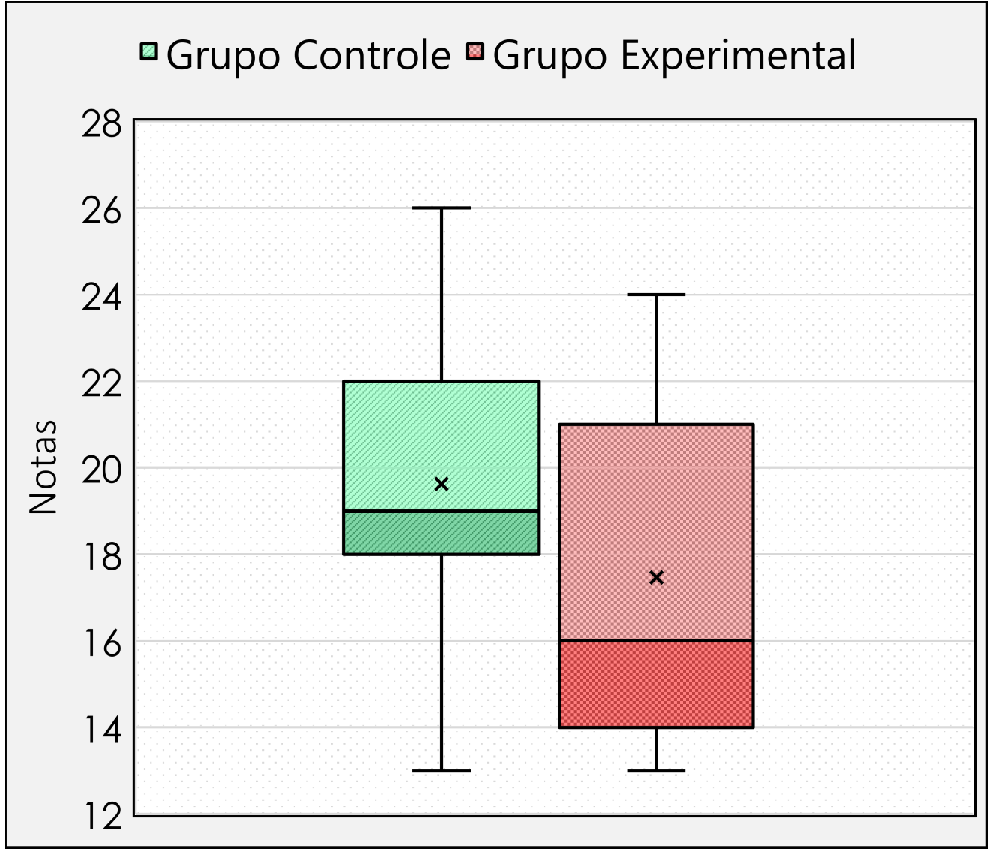
\includegraphics[width=\linewidth]{./Visuais/CaixaEstreitaEnfeitado.pdf}
    \legend{Fonte: Elaborada pelo autor (2021).}
  
\end{figure}



\begin{figure}[htb]

    \caption{\label{fig:barrasExp}Gráfico de Barras da taxa de acerto por questão no pré-teste (Grupo Experimental)}
    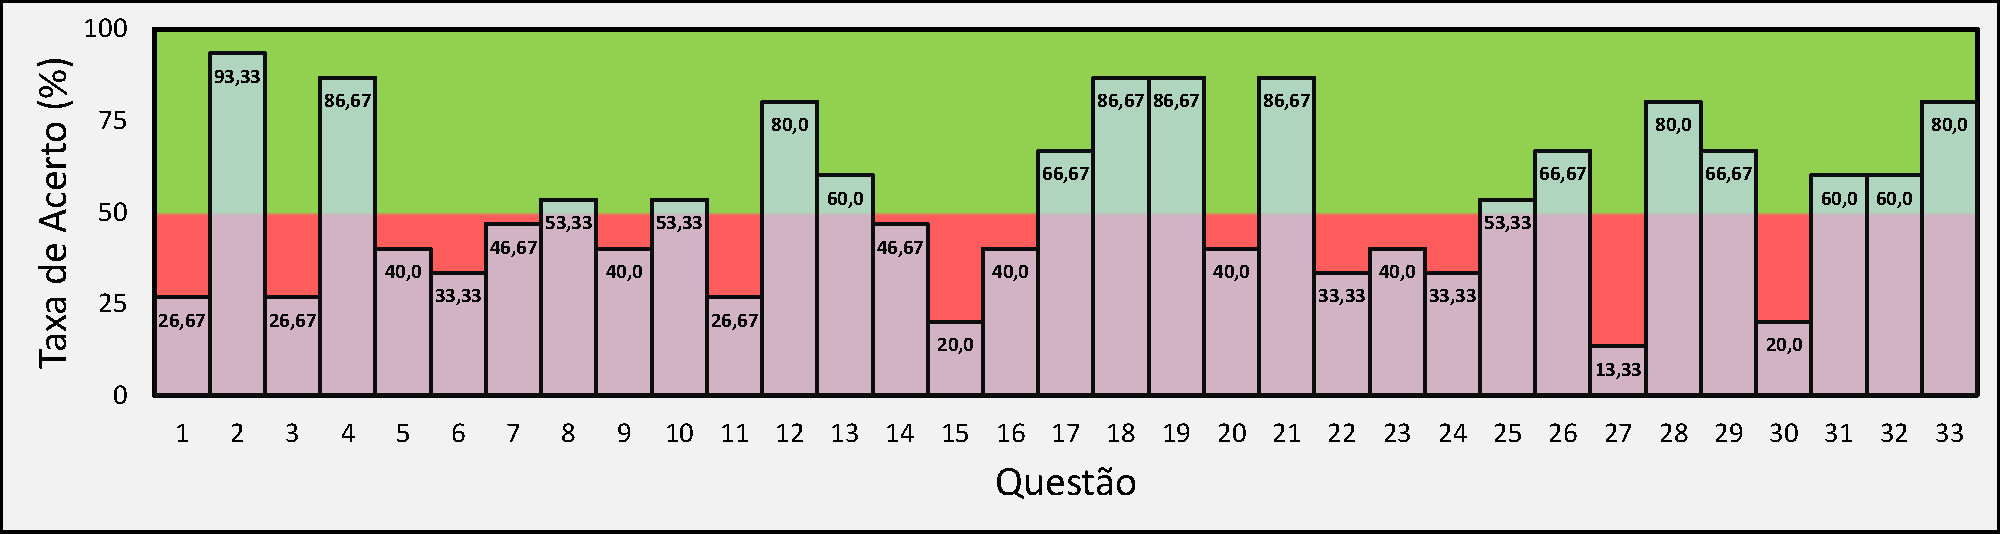
\includegraphics[width=\linewidth]{./Visuais/Notas3.pdf}
    \legend{Fonte: Elaborada pelo autor (2021).}
  
\end{figure}

\begin{figure}[htb]

    \caption{\label{fig:barrasCon}Gráfico de Barras da taxa de acerto por questão no pré-teste (Grupo Controle)}
    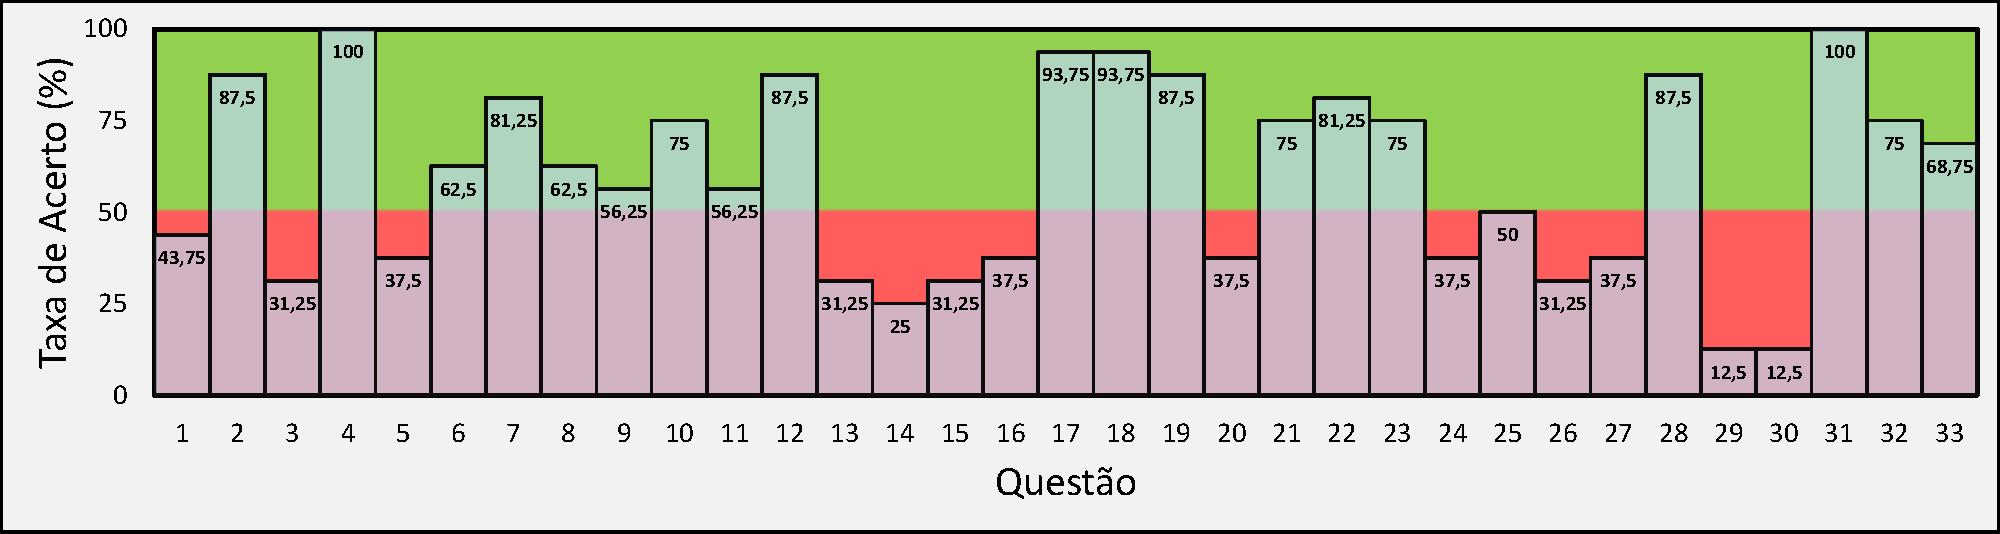
\includegraphics[width=\linewidth]{./Visuais/Notas4.pdf}
    \legend{Fonte: Elaborada pelo autor (2021).}
  
\end{figure}


\begin{figure}[htb]

    \caption{\label{fig:normal}Distribuição das notas atingidas no pré-teste}
    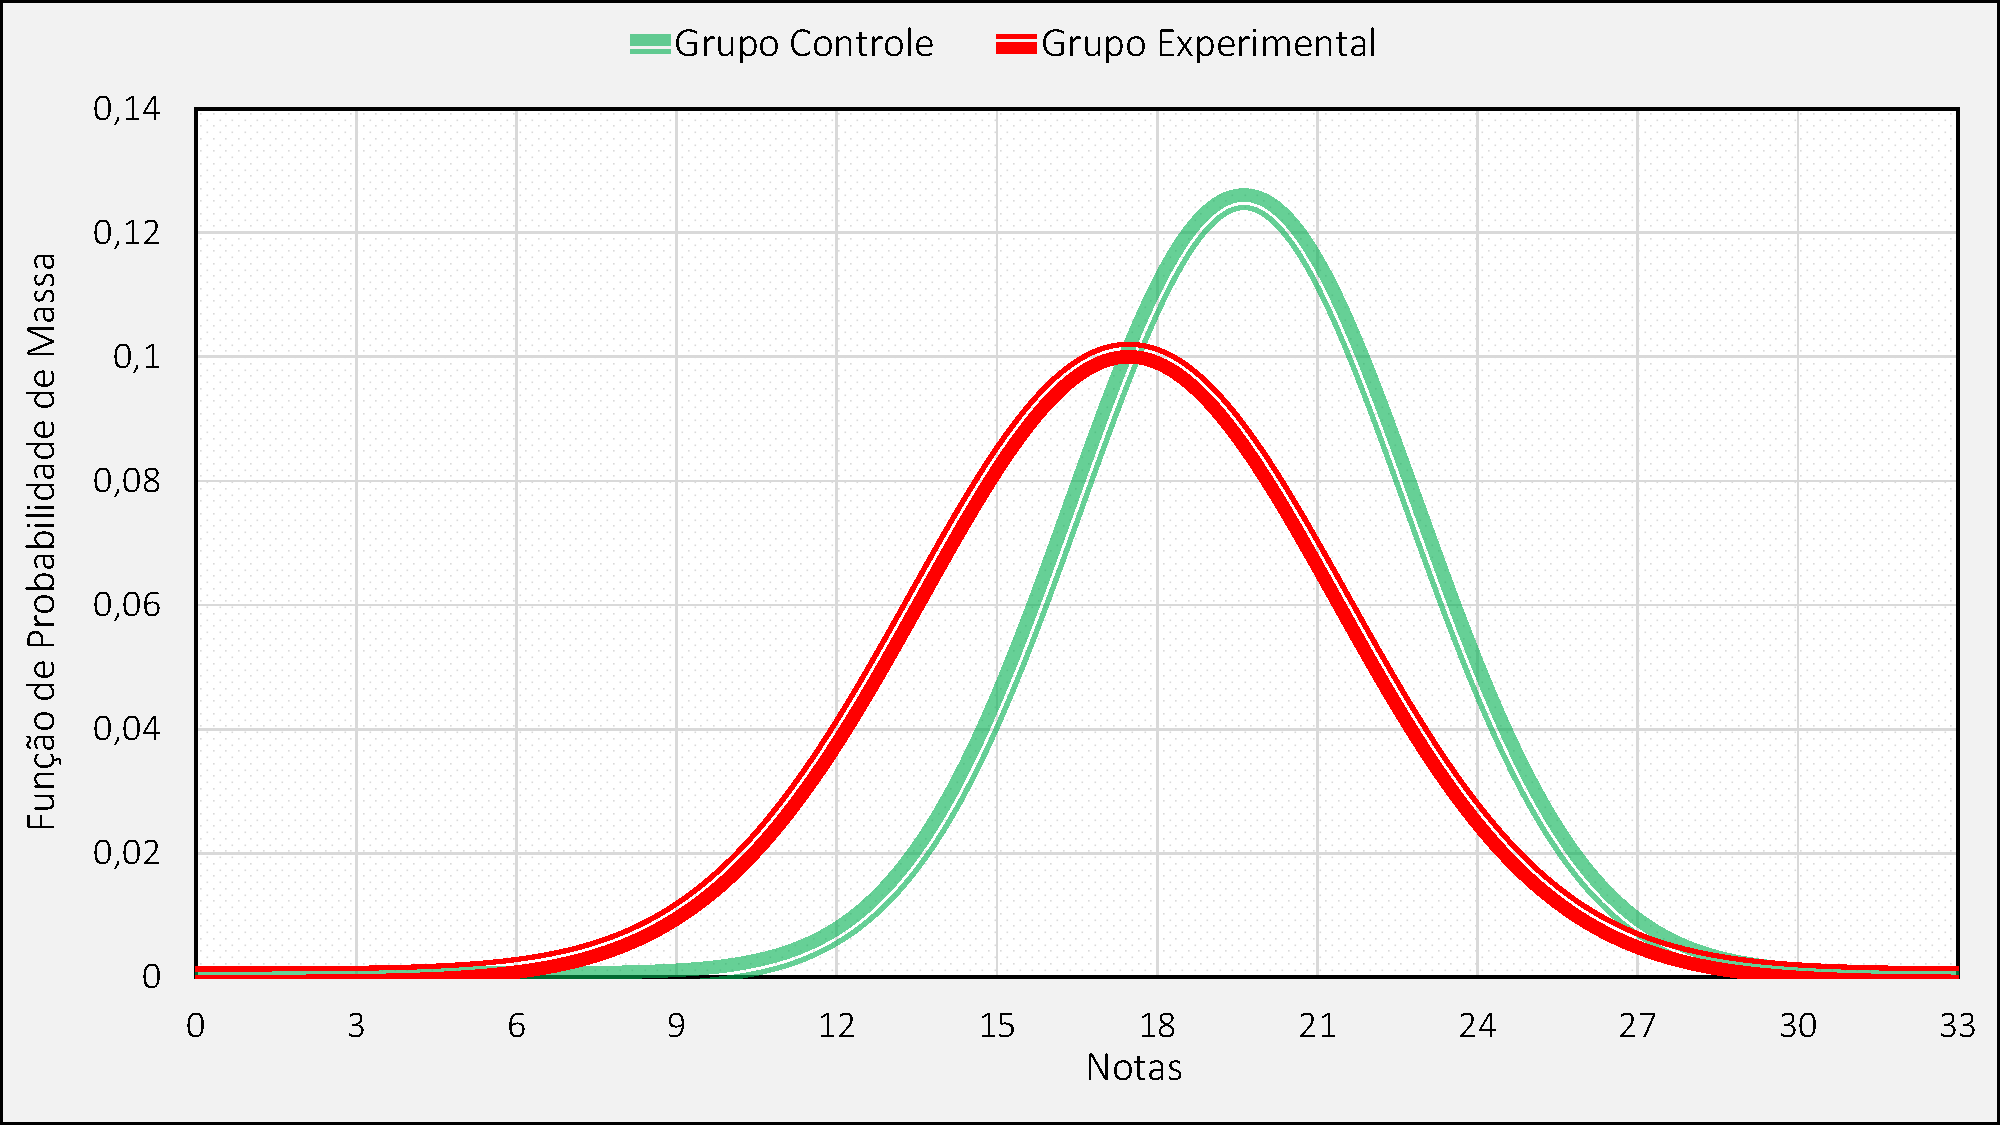
\includegraphics[width=\linewidth]{./Visuais/Graficos1.pdf}
    \legend{Fonte: Elaborada pelo autor (2021).}
  
\end{figure}